\chapter{Abstract}
Human-robot interaction (HRI) has been a topic of both science fiction and academic speculation even before any robots existed \cite{7}. HRI research is focusing to build an intuitive and easy communication with the robot through speech, gestures, and facial expressions. The use of hand gestures provides an attractive alternative to complex interfaced devices for HRI. In particular, visual interpretation of hand gestures can help in achieving the ease and naturalness desired for HRI. This has motivated a very active research concerned with computer vision-based analysis and interpretation of hand gestures. Important differences in the gesture interpretation approaches arise depending on whether 3D based model or appearance based model of the gesture is used. 

In this thesis, we attempt to implement the hand gesture recognition for robots by modeling, training, analyzing, and recognizing gestures by using computer vision and machine learning techniques. Additionally, 3D based gesture modeling with skeletal points tracking will be used. On the one side, gestures will be used command the robot to execute certain actions and on the other side gestures will be translated and spoken out by the robot.

We further hope to provide a platform to integrate Sign Language Translation to assist people with hearing and speech disabilities. However, further implementations and training data are needed to use this platform as a full fledged Sign Language Translator.

\subsection*{Keywords} Human-Robot Interaction, HRI, Computer Vision, Depth Camera, Hand Gesture, 3D hand based model, Skeleton tracking, Gesture Recognition, Sign Language Translation, Hidden Markov Model, NAO

\chapter{Motivation} Huge influence of computers in society has made smart devices, an important part of our lives. Availability and affordability of such devices motivated us to use them in our day-to-day living. The list of smart devices includes personal automatic and semi-automatic robots which are also playing a major role in our household. For an instance, Smart Vacuum Cleaner is a robot that automatically cleans the floor and goes to its charging station without human interaction.

Interaction with smart devices has still been mostly through displays, keyboards, mouse and touch interfaces. These devices have grown to be familiar but inherently limit the speed and naturalness with which we can interact with the computer.  Usage of robots for domestic and industrial purposes has been continuously increasing. Thus in recent years, there has been a tremendous push in research toward an intuitive and easy communication with the robot through speech, gestures, and facial expressions.

Tremendous progress had been made in speech recognition and several commercially successful speech interfaces are available. However, there has been an increased interest in recent years in trying to introduce other human-to-human communication modalities into HRI. This includes a class of techniques based on the movement of the human arm and hand, or hand gestures. The use of hand gestures provides an alternative mode of communication for Human-robot interaction than the conventional cumbersome devices.

\begin{figure}
	[h] \centering 
	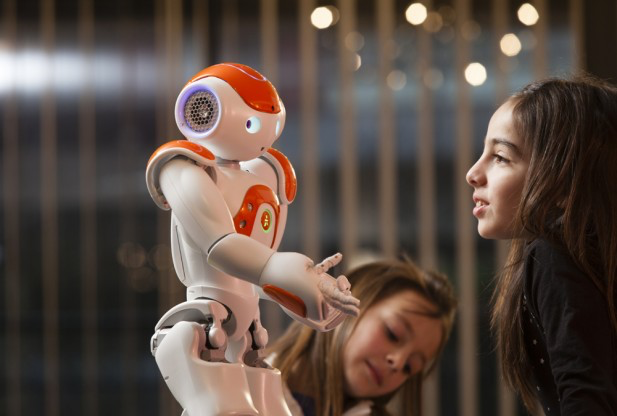
\includegraphics[width=5.5cm]{figures/nao-interaction.png} 
	\caption{Human Robot Interaction by Aldebaran Robotics} 
	\label{fig:nao:interaction} 
\end{figure}

\chapter{Background} 
\section{Robot and Artificial intelligence} Proper vision is the utmost importance for the function of any vision based autonomous robot. Areas of artificial intelligence deal with autonomous planning or deliberation for robotic systems to navigate through an environment. A detailed understanding of these environments is required to navigate through them. High-level information about the environment could be provided by a computer vision system that is acting as a vision sensor.

Computer vision is a field that includes methods for acquiring, processing, analyzing, and understanding images and, in general, high-dimensional data from the real world in order to produce numerical or symbolic information, e.g., in the forms of decisions \cite{1}.

In this thesis, we will focus on the hand gesture recognition using computer vision techniques for a humanoid robot named as NAO, as shown in the figure \ref{fig:nao}. NAO is an autonomous, programmable humanoid robot developed by Aldebaran Robotics. The NAO Academics Edition was developed for universities and laboratories for research and education purposes. Table \ref{tb:nao} shows the specification of NAO according to Aldebaran Robotics.
\begin{table}
	[h] \centering \caption{NAO's hardware and software specification } \label{tb:nao} 
	\begin{tabular}
		{|l|l|} \hline Height & 58 centimetres (23 in) \\
		\hline Weight & 4.3 kilograms (9.5 lb) \\
		\hline Autonomy & 60 minutes (active use), 90 minutes (normal use) \\
		\hline Degrees of freedom & 21 to 25 \\
		\hline CPU & 2 x Intel Atom @ 1.6 GHz \\
		\hline Built-in OS & Linux \\
		\hline Compatible OS & Windows, Mac OS, Linux \\
		\hline Programming languages & C++, Python, Java, MATLAB, Urbi, C, .Net \\
		\hline Vision & 2 x HD 1280x960 cameras \\
		\hline Connectivity & Ethernet, Wi-Fi \\
		\hline \multirow{6}{*}{Sensors} & 4 x directional microphones \\
		& 1 x sonar rangefinder \\
		& 2 x IR emitters and receivers \\
		& 1 x inertial board \\
		& 9 x tactile sensors \\
		& 8 x pressure sensors \\
		\hline 
	\end{tabular}
\end{table}

\subsection{NAO Vision} Two identical video cameras are located in the forehead of NAO. They provide up to 1280x960 resolution at 30 frames per second. They can be used to identify objects in the visual field such as goals and balls, and bottom camera can ease NAO's dribbles. NAO contains a set of algorithms for detecting and recognizing faces and shapes. NAO can recognize who is talking to it or find a ball or, eventually, more complex objects.

\subsection{Extending NAO with Depth Camera} 
3D cameras such as Microsoft Kinect and Asus Xtion are used not only for gaming but also for analyzing 3D data, including algorithms for feature selection, scene analysis, motion tracking, skeletal tracking and gesture recognition. 

In this thesis, we focus on using Asus Xtion as an external hardware as shown in the figure \ref{fig:xtion}, due to the computational limitations of the NAO to process the images from two inbuilt hd stereo cameras, that ultimately makes NAO incapable of doing an efficient gesture recognition in real time.

\begin{figure}
	\centering
	\begin{minipage}{.5\textwidth}
		\centering
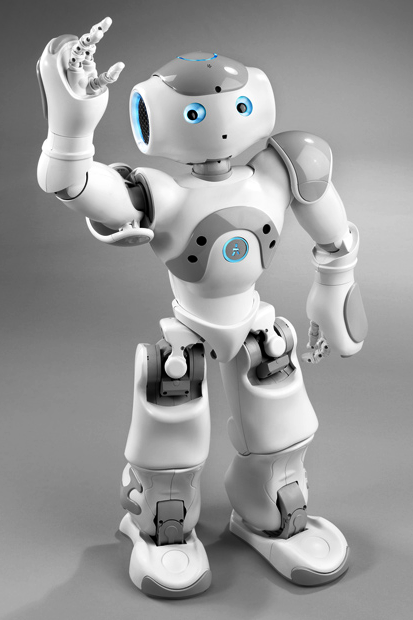
\includegraphics[height=7cm]{figures/nao.png} 
		\captionof{figure}{NAO}
		\label{fig:nao}
	\end{minipage}%
	\begin{minipage}{.5\textwidth}
		\centering
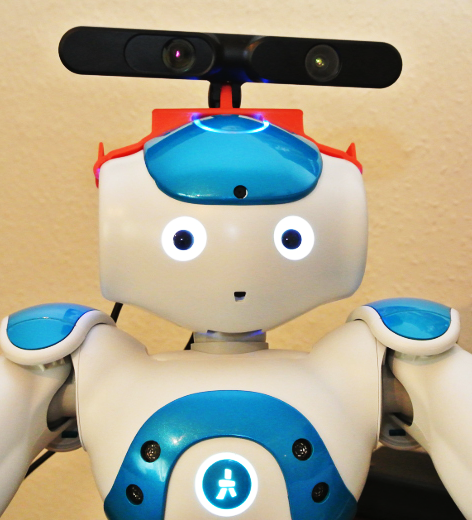
\includegraphics[height=7cm]{figures/nao-xtion.png} 
		\captionof{figure}{Asus Xtion mounted on NAO }
		\label{fig:xtion}
	\end{minipage}
\end{figure}


\section{Hand Gesture} Human hand gestures are a means of non-verbal interaction among people. They range from simple actions of using our hand to point at, to the more complex ones that express our feelings and allow us to communicate with others. To exploit the use of gestures in HRI, it is necessary to provide the means by which they can be interpreted by robots. The HRI interpretation of gestures requires that dynamic and/or static configurations of the human hand, arm, and even other parts of the human body, be measurable by the machine \cite{6}. 

\section{Hand Gesture Recognition} Initial attempts to recognize hand gestures resulted in electro-mechanical devices that directly measure hand and/or arm joint angles and spatial position using sensors \cite{3}. Glove-based gestural interfaces require the user to wear such a complex device that hinders the ease and naturalness with which the user can interact with the computer controlled environment. 

Even though such hand gloves are used in highly specialized domain such as simulation of medical surgery or even in the real surgery, the everyday user will be certainly deterred by such sophisticated interfacing devices. As an active result of the motivated research in HRI, computer vision based techniques were innovated to augment the naturalness of interaction.

\subsection{Gesture Modeling} Figure \ref{fig:ges:model} shows various types of modeling techniques used for Gesture modeling \cite{3}. Selection of an appropriate gesture modeling depends primarily on the intended application. For an application that needs just hand gesture to go up and down or left and light, a very simple model may be sufficient. However, if the purpose is a natural-like interaction, a model has to be sophisticated enough to interpret all the possible gesture. The following section discusses various gesture modeling techniques which are being used by the existing hand gesture recognition applications. 

\begin{figure}
	[h] \centering 
	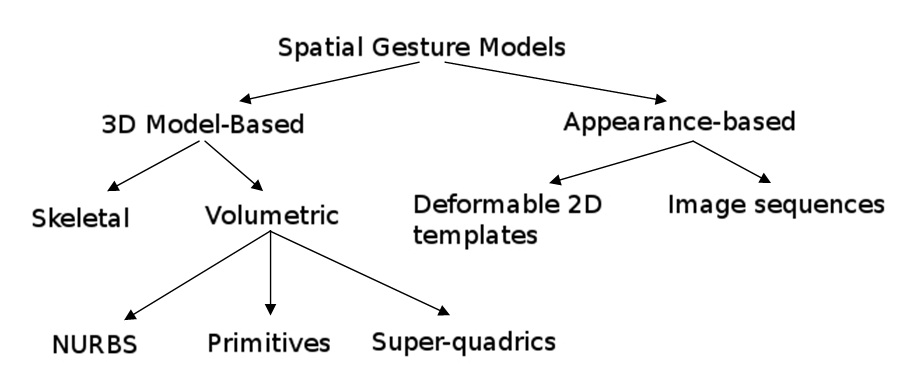
\includegraphics[height=5cm]{figures/ges-model.png} 
	\caption{Different gesture modeling} 
	\label{fig:ges:model} 
\end{figure}

Appearance based models don't use the spatial representation of the body, because they derive the parameters directly from the images or videos using a template database. 

3D hand based model approach uses volumetric or skeletal models, or even a combination of  both. Volumetric approaches have been heavily used in computer animation industry and for computer vision purposes. The models are generally created of complicated 3D surfaces. The drawback of this method is that is very computational intensive. 

Instead of using intensive processing of the 3D hand models and dealing with a lot of parameters, one can just use a simplified version that analyses the joint angle parameters along with segment length. This is known as a skeletal representation of the body, where a virtual skeleton of the person is computed and parts of the body are mapped to certain segments \cite{4}. The analysis here is done using the position and orientation of these segments and the relation between each one of them.

In this thesis, we focus on Skeletal based modeling algorithms which are faster because the detection program has to focus only on the significant parts of the body. Moreover, it allows to do pattern matching against a template database. 

\subsection{Gestural Taxonomy }
Several alternative taxonomies have been suggested that deal with psychological aspects of gestures \cite{3}. All hand/arm movements are first classified into two major classes as shown in the figure \ref{fig:ges:tax}.

\begin{figure}
	[h] \centering 
	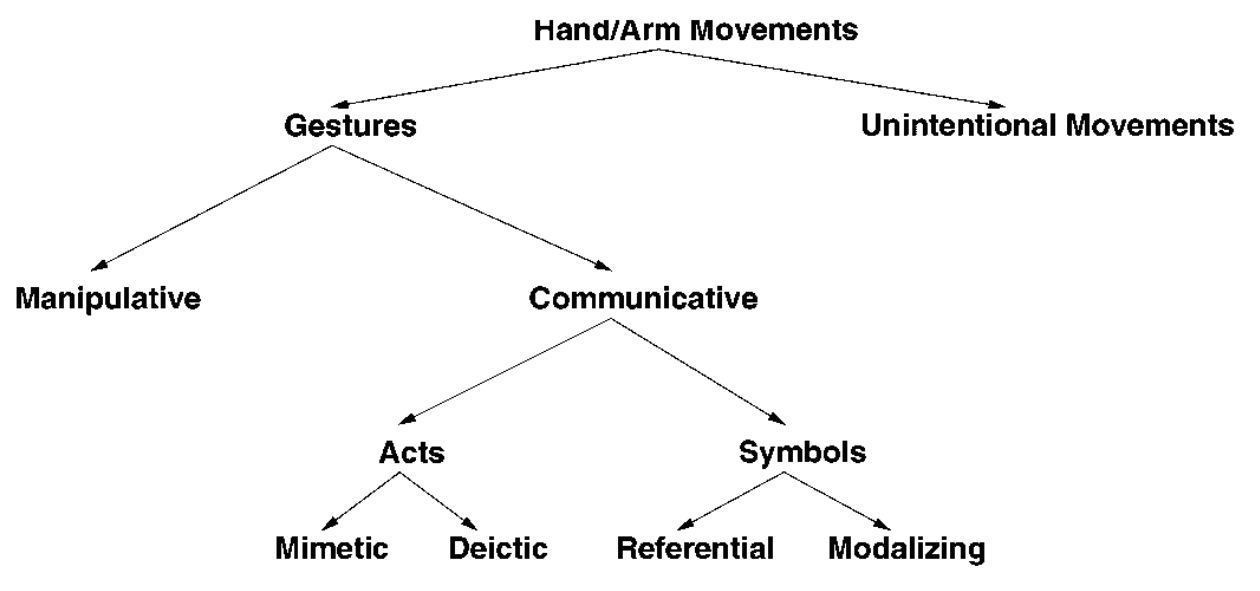
\includegraphics[width=13cm]{figures/ges-tax.png} 
	\caption{Different gesture modeling} 
	\label{fig:ges:tax} 
\end{figure}

Manipulative gestures are the ones used to act on objects. For example, moving a chair from one location to another. Manipulative gestures in the context of HRI are mainly developed for medical surgery. Communicative gestures, on the other hand, have purely communicational purpose. In a natural environment they are usually accompanied by speech or spoken as a sign language. In HRI context these gesture are one of the commonly used gestures, since they can often be represented by static as well as dynamic hand postures.

In this thesis, we focus on communicative gestures in the form of symbols. They symbolize some referential action. For instance, circular motion of hand may be referred as an alphabet "O" or as an object such as wheel or as a command to turn in a circular motion .


\subsection{Gesture Recognition}
The task of gesture recognition shares certain similarities with other recognition tasks, such as speech recognition and biometrics. Though alternatives such as DP-matching algorithms have been attempted, the most successful solutions involves feature-based statistical learning algorithm, usually Hidden Markov Models \cite{5}. 

In this thesis, we focus on the recognition using  machine learning technique based on hidden Markov model. HMM is a statistical model in which the system being modeled is assumed to be a Markov process with unobserved (hidden) states. In simpler Markov models, the state is directly visible to the observer and therefore the state transition probabilities are the only parameters. In a hidden Markov model, the state is not directly visible, but output dependent on the state is visible.


\chapter{Goal} As described earlier, HRI research is focusing to build an intuitive and easy communication with the robot through speech, gestures, and facial expressions. The use of hand gestures provides the ease and naturalness with which the user can interact with robots.

In this thesis, we attempt to implement the feature for NAO to recognize hand gestures and execute predefined actions based on the gesture. NAO will be extended with an external depth camera, that will enable NAO to recognize 3D hand based modeled gestures. This 3D camera will be mounted on the head of NAO, so that it can scan for gestures in the horizon. Additionally, skeletal points tracking algorithm with machine learning technique using Hidden Markov Models will be used to recognize the gestures. With the hand gesture recognizing feature, NAO will be available to the users in two modes.

\begin{itemize}
	\item \textbf{Command mode:} In this mode, a gesture will be recognized by NAO and related task will be executed. Even though the gesture based interaction is real time, NAO can not be interrupted or stopped by using any gesture while it is executing a task. However, part of NAO intelligence such as voice commands can be used in such situation to stop or interrupt the ongoing task execution.
	\item \textbf{Translation mode:} In this mode, NAO will be directly translating the meaning of the gesticulated gestures. To achieve this, text-to-speech library of NAO will be used and recognized gesture can be spoken out using the integrated loud speaker. In future, it will allow NAO to translate a sign language to assist people with hearing and speech disabilities.
\end{itemize}

In this thesis, we planned to train NAO with few very simple gestures due to the reason that NAO has limited resources. Gestures will involve both the hands or single hand to interact with the robot.

\chapter{Approach} The figure \ref{fig:flow} shows the flow diagram of hand gesture recognition system that is going to implemented in this project work. Each block contains different software components that are executed sequentially. However, training phase must be carried out before this system is available for recognition. Finally, these components will be integrated into NAO.

\begin{figure}
	[!h] \centering 
	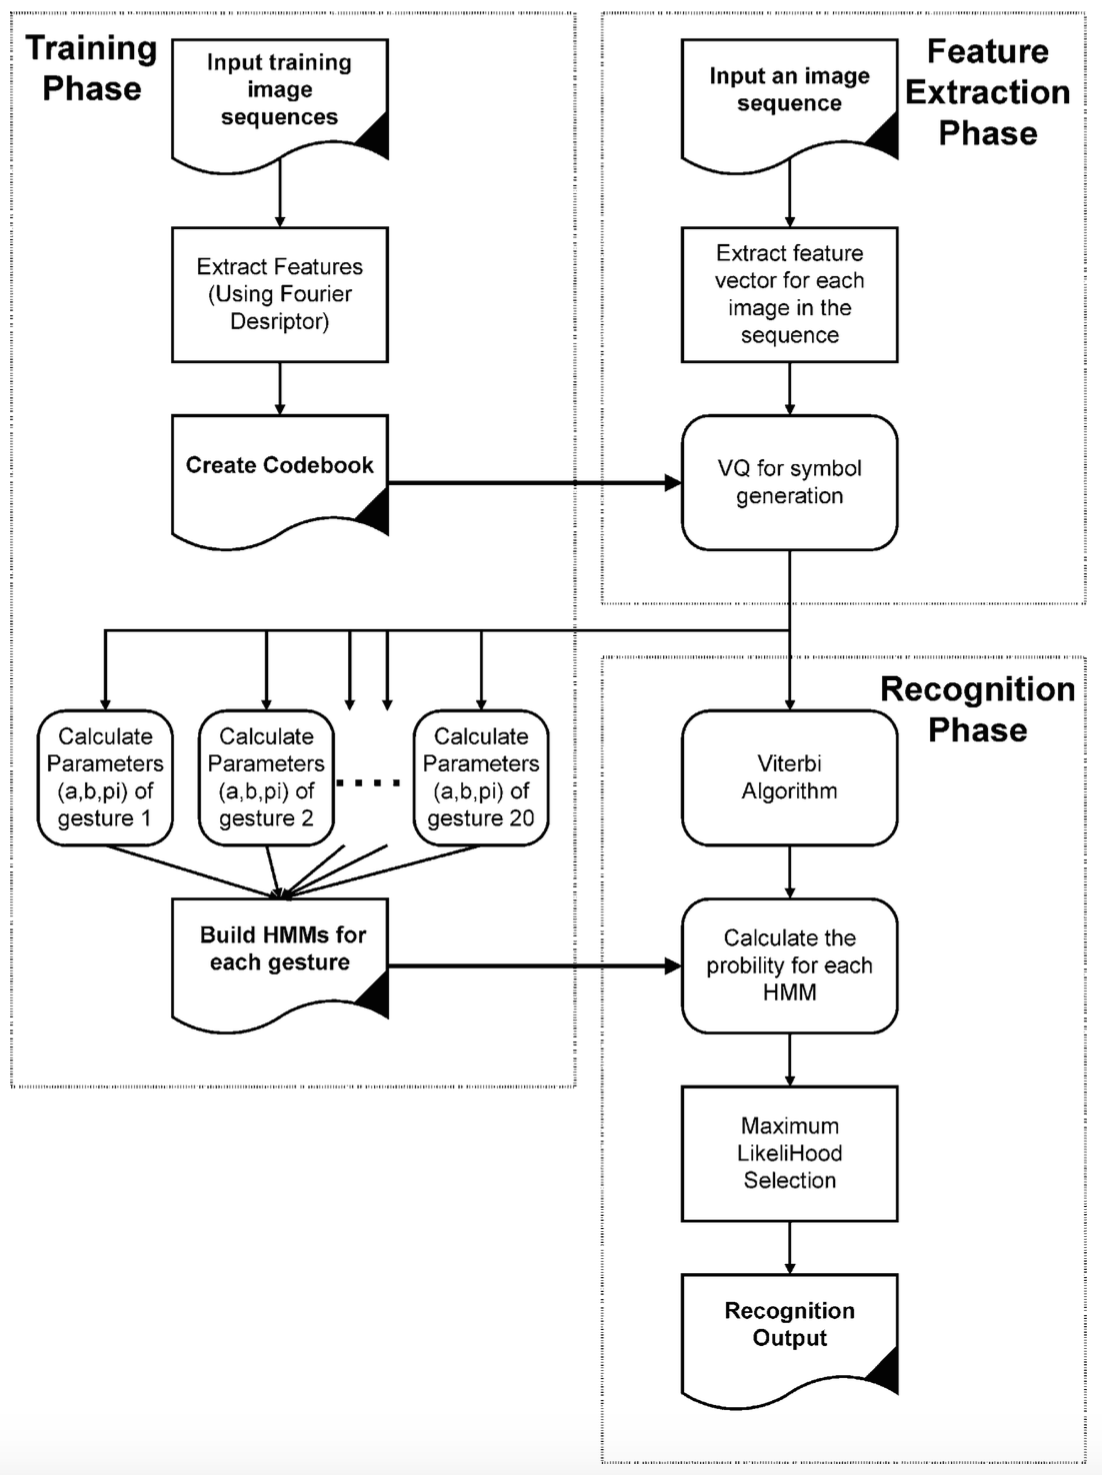
\includegraphics[width=9cm]{figures/flow.png} \caption{Flow diagram of hand gesture recognition system} \label{fig:flow} 
\end{figure}

\section{Sensing} 
3D camera records 30 frames of color image as well as depth image per second and outputs as a data package. Figure \ref{fig:depth} shows the single frame of depth image taken from Microsoft Kinect where darker gray values represent the farther distance and lighter gray values represent the closer distance from the camera.

\begin{figure}
	\centering
	\begin{minipage}{.5\textwidth}
		\centering
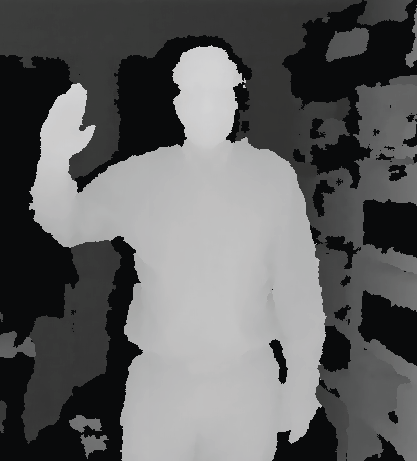
\includegraphics[height=7cm]{figures/depth.png} 
		\captionof{figure}{Depth image of 3D Camera}
		\label{fig:depth}
	\end{minipage}%
	\begin{minipage}{.5\textwidth}
		\centering
		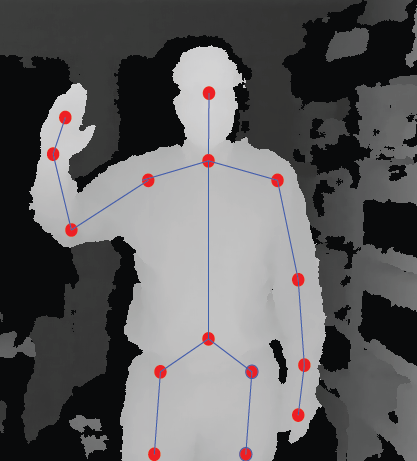
\includegraphics[height=7cm]{figures/depth-skeleton.png}
		\captionof{figure}{Skeleton tracking }
		\label{fig:skeleton}
	\end{minipage}
\end{figure}

\section{Feature Extraction}
Output package from sensor data will be inputted to feature detection and extraction unit. OpenNI is a software component that will track the anatomical landmarks of the human body from the package and extract significant joint angle parameters along with segment length and present them three dimensionally as shown in the figure \ref{fig:skeleton}. Finally, only joints of both the arms will be picked out from the array of features, since it will be the significant joints needed for hand gesture recognition.

\section{Modeling and Classification}
In order to use this hand recognition system, all chosen gestures must be observed and the system must be trained. Therefore, a set of simple gestures will be chosen and observed for training. Each gesture is isolated in time and gesticulated for certain duration. However, sensors provides 30 frames of discrete states of gesture per second. 

For example, a gesture is gesticulated by simply drawing a circle in the air and its ideal states are shown in the figure \ref{fig:ges:state}. It will be modeled as a position of hand passing through 8 states of the circle. Each state is a point in space with x, y and z axis data. This approach makes it possible for us to reduce our observation data to sequential 3D points and focus on the recognition task without processing all those pixels. Each trained model can then be used to determine with what probability a given gesture appears in test data. Therefore, the trained Hidden Markov models will be used to recognize gestures \cite{2}. 

\begin{figure}
	\centering
	\begin{minipage}{.3\textwidth}
		\centering
		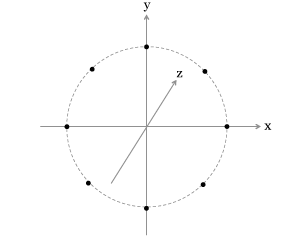
\includegraphics[width=6cm]{figures/ges-states.png}
		\captionof{figure}{HMM States of circular gesture}
		\label{fig:ges:state}
	\end{minipage}%
	\begin{minipage}{.7\textwidth}
		\centering
		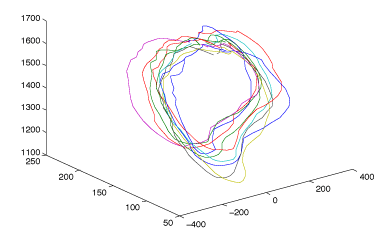
\includegraphics[width=10cm]{figures/ges-train.png}
		\captionof{figure}{Observations of circular gestures}
		\label{fig:ges:train}
	\end{minipage}
\end{figure}

\section{Gesture Analysis and Recognition}
This step contains the analysis of gesticulated gesture and finding out the likelihood of that gesture with trained data, known as gesture recognition. Figure \ref{fig:ges:train}  contains colored rings of noisy data of gestures that represent instances of a real circle gesture. Sensing and feature detection module will produce 60 observations of the circle gesture for 2 seconds, since the depth camera records at 30 frame per second. To decide whether a given set of 60 observations contains a circle gesture, we need to first determine the likelihood that the hand passed through the eight states of the gesture in the expected sequence.

Discrete HMM is a finite set of M possible output symbols and a sequence of N hidden states which reveal some probability. To reduce our real gesture data to a workable number of discrete output symbols and states, we can use any clustering algorithm to cluster the 3D points of all our training data of circle gesture into clusters and label them. That is to say, every point in the training data represents an output symbol that is closely tied to one of the 8 true states of the model.

Looking at the labeled data, we can estimate how likely it is that a hand passed through the 8 clusters in the same sequence as a circle gesture, and if the likelihood is high enough, then the gesture is considered to be recognized.

\begin{figure}
	[h] \centering 
	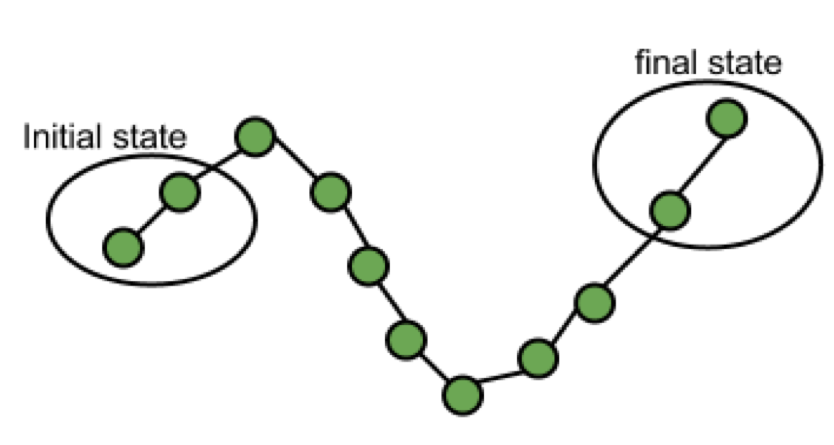
\includegraphics[height=7cm]{figures/ges-rec.png} \caption{shows the states of Arabic sign language to convey "Hello". It is consisted of 11 states of Markov models and if there is higher likelihood of the hand position passed through states sequentially from initial to final, then it is recognized as "Hello".} \label{fig:ges:reg} 
\end{figure}

\section{Human-Robot Interaction}
Finally, the recognized gesture will be interpreted by NAO to execute an specified task. The motion of NAO will be defined by the application Choregraphe in Command Mode. For example. circle gesture would ask NAO to turn around. However, NAO will also be available in Translation Mode by using ALTextToSpeech Library to translate the recognized gesture.


\chapter{Schedule}
\begin{itemize}
	\item \textbf{October - Preparation:} This includes the analysis of relevant papers as well as the consideration of the already available components.
	\item \textbf{November - Setup:} Software and Hardware environment setup. Getting to know the tools that will be used during this project work.
	\item \textbf{December / January - Implementation:} Proposed functionalities will be implemented.
	\item \textbf{January / February - Testing:} This includes testing, bug fixing and improvising the implementation.
	\item \textbf{February / March - Documentation:} This includes the documentation of the code and writing up the thesis.
\end{itemize}

\chapter{Details}
\begin{itemize}
	\item Language of the Master Thesis: English
	\item Document processing system: LaTex with TexStudio
	\item Operating system: Linux Ubuntu, Mac OS X
	\item Software components: OpenNI, OpenCV, NAO Choregraphe
	\item Hardware components: NAO, Asus Xtion
	\item Programming Language: C++, Python
	\item Version control system: Git
	\item Advisor: Dr. Yuan Xu
	\item Professor: Prof. Dr. Sahin Albayrak
\end{itemize}
